\chapter{Analysis of Twitter's Social Structure}


Stuff to add to this section:
\begin{itemize}
\item Change tweet features for each simulation and make comparison on these differences
\item Observe differences in patterns when network generation parameters are altered
\item Link up section to previous section (i.e. how did the previous research help and how does this build on that work?)
\item Explain how this section becomes the basis for work in 'main chapter 3'.
\item (e.g. Issues with current method (too long, requires network, inaccurate due to having to choose users with fewer followers), so need a quicker, more accessible and online approach).
\item Explain the Mechanical Turk questions in more detail, with examples.
\item Discuss about the machine learning approach used (logistic regression and how it works)
\item Link 'retweet volume' to 'retweet group size'
\end{itemize}

Twitter is often seen as one of the biggest sources of new and live information on the Internet, with millions of people producing and absorbing information daily. Users receive tweets onto their timelines from the users that they follow. Thus, a user has some control over the \textit{type} of information they receive by choosing which other users to follow. A particular user, therefore, may not be aware of information that exists outside of their local network, since he or she is not directly exposed to the information produced by non-followees.
\\
Retweeting allows users to forward information they receive onto their own followers. As a result, followers of these users, who might not normally be exposed to this information, now have a chance to access it. A user who decides to retweet a tweet can be said to consider that tweet to be \textit{interesting} (at least, to their followers), since that user has taken the time to read the tweet, decided whether or not to share it, and then to actually retweet it \cite{uysal11}.
\\
Several factors can affect a user's decision to retweet, such as whether the tweet contains an (interesting) URL, whether the tweet mentions another user, whether a user even has a chance to see the tweet, the influence of the author, and so on. These factors account for a user's individual retweet \textit{decision} on a particular tweet, and the combination of several users' retweet decisions dictate how far the tweet will propagate. However, it is our belief that the social network structure also has an affect on how far tweets can travel.
\\
The social structure of Twitter is built up by users electing to follow other users. When a user follows a user, a directional link is forged between them, and any tweets generated, or forwarded, by the followed user are passed down the link. It's clear to see that, as more links are made between users, many more avenues are generated for message propagation throughout the social structure. Users with a high in- and out-degree can become an information highway, but users with a low out-degree are a bottleneck of information. 
\\
In this chapter, we demonstrate how different network types support different propagation characteristics through the use of a model simulating each network type. Using the model, we make predictions on the retweet outcomes on several network types, and compare these to the characteristics of the propagation in real Twitter networks. We finish by discussing how the \textit{interestingness} of a tweet may be inferred from simulating the network in this way.

\section{Background to This Area}
\cite{uysal11} discusses an idea similar to that of predicting the interestingness of a tweet, but focuses mainly on predicting the users most likely to find the tweet interesting enough to retweet. Similarly, \cite{hong11} looks at the same issue, but at the other way around by predicting the \textit{type} of tweets that are likely to be retweeted many times. Discussions on the retweet decision in relation to a user's recognition of its features take place in \cite{chorley12} as well as conclusions about the effect of features such as the number of followers of a user or any pre-existing metadata on the interestingness of the tweet.
\\
The notion of time decay and how this is associated with a user's retweet decision is discussed in addition to a retweet probability prediction in \cite{zhu11} (and \cite{peng11}), which is the basis of the model we use in this paper.

\section{Overview}
In the next sections, we introduce and briefly explain the regression model we use for simulations and predictions. We then go on to analyse the differences in the propagation characteristics between three different network types before comparing the results of simulations on these networks with data collected from the Twitter social graph. We finish by introducing a methodology for predicting the interestingness of a particular tweet to a particular user and how this might be improved.
\\
Ideally, there are two things we'd like to see from the first set of experiments; firstly, that changing the network type and properties does, indeed, affect the propagation behaviour, and, secondly, that at least some of the results from the experimentation correspond to Twitter's own retweet behaviour so that a fair comparison and justifications of our results can be made.
\\
With regard to our prediction work, we'd like to be able to make relatively decent predictions on which tweets are of interest, and which are not, based on the simulation research in the next section.

\section{Model} 
As mentioned above, \cite{zhu11} introduced and discussed their prediction model, which was shown to perform well when predicting the retweet decision of a user. Their model trains a logistic regression using a set of user-, tweet- and context- features in order to classify an experimental tweet and output a retweet probability based on a set of features.

\subsection{Machine Learning}
Machine learning techniques are useful for making predictions based on certain input criteria based on the perceived history of previous outputs from the same inputs. 

\subsubsection{General Overview}
For example, consider the three attributes, A, B and C, each of which is of a boolean data type. A machine learning technique is `shown' that in every case where A is True and B is False, then C is true; and that in each case where A is False and B is True, then C becomes False. The history of these inputs suggests that A is strongly associated with C (the strength of this relationship will increase if the input/output history is larger), such that if the technique now tries to predict C based on the fact that A = True, then it will likely suggest that C is also True with high confidence.
\\ \\
A technique that has been shown many of these input/output combinations (known as `instances') is said to be a trained model, where the model type is that of the learning technique used. This model can then make predictions based on the same inputs it has been trained on, and will therefore not work for attribute inputs that it hasn't been trained with.
\\
Generally, in large enough datasets, the training data will not exclusively contain instances where A is the inverse of B, and so the model will be able to make predictions in cases where A = B (though if these cases are less prevalent then the confidence of these prediction outputs will be weaker). When training the model, instances must contain the input attributes as well as the value of the output attribute. When testing against the model after training, the model is supplied the input attributes and predicts the value of the output attribute. Generally, the model will also indicate how confident it feels that the prediction is correct, and thus an idea can be obtained of the value of each of the input attributes. Some model types (particularly regressions) output instead the \emph{probability} with which the attributes align to the trained regression.
\\ \\
In this example the focus has been on boolean data types, but most machine learning techniques are not limited to these. Indeed, most applications require the learning of real numbers (integers, floats, etc.) and more highly-dimensioned nominal attributes, where there are several categories that the value of one of the input attributes can lie in. Many machine learning techniques exist and some are more accurate than others when it comes to different data types and several support the notion of `weighting' attributes, in which a strength weight is assigned to each attribute to signify the confidence with which the model should rely on that attribute for producing the prediction.
\\
For example, for purely nominal values, then logistic regressions can be accurate in predicting outcomes, whereas for a mixture of real and nominal attributes a Bayesian attempt might be more suitable. 

\subsubsection{Logistic Regression} 
The work in this chapter utilises a logistic regression for outputting retweet predictions based on the feature input criteria discussed later.
\\
As mentioned, the logistic regression predicts the statistical likelihood that the input features align with what the model has been trained with. The work in this chapter relies on the use of a retweet probability of a given user acting on a given Tweet at a certain time. Thus, it is trained in such a way so that the binary input attributes produce a binary output retweet outcome attribute: 1 for retweet, 0 for no retweet.
\\
When testing, the binary features of the test set are used to output the probability that these features will result in a retweet.

\subsection{Algorithm}
Include image indicating the flow of events that take place for the model
\\
Pseudocode for the algorithm
\\
In essence, the model requires a network of users and one tweet to start the simulation. It starts by initialising a user set, \textit{U}, to contain one source user from the network, $U_s$. This source user then transmits a tweet which is then received by its followers. $U_s$ is then removed from $U$. For each follower, its tweet and user features are classified to produce a retweet probability. If this is greater than a random number, $R$, then the user retweets the tweet to its followers and the process repeats. Any user that retweets the tweet is removed from $U$ and added to the retweet decision set $RT$. The followers of the retweeter are added to $U$ for the next iteration, in which each user in $U$ has received the tweet onto their timeline. The retweet volume of this tweet in this network is then the cardinality of the set $RT$.

\subsubsection{Twitter Timelines}
A tweet in a user's timeline will slip further down in the timeline as time goes by. This happens whether the tweet is interesting or not and whether or not the user has even seen the tweet.  Users having a quick browse through Twitter may not have time to scroll down to find these interesting tweets (and will not know they exist) and thus tweets left in the timeline have their retweet chance decay over time.
\\
We emulate this phenomenon in our simulations by removing the tweet from a user's timeline (by removing the user from the set $U$) if the user has not retweeted the tweet within a timestep threshold, which can be varied to alter the volatility of the retweet.

\subsection{Features}
We use this model as part of a simulator in order to obtain an approximate retweet volume of each tweet when the retweet probabilities of each user receiving the tweet are combined. \cite{zhu11} used a set of around 50 features, though they mention how some features have more weight than others. In order to simplify the simulation significantly and to make data collection more tractable, we decided to use only the following four major features;
\begin{itemize}
\item \emph{follows} - Whether or not the user exposed to the tweet is a follower of the author;
\item \emph{followed} - Whether or not the user exposed to the tweet is followed by the author;
\item \emph{mentioned} - Whether or not the user exposed to the tweet is mentioned in the tweet;
\item \emph{URL} - Whether or not the tweet contains a URL;
\end{itemize}
Where \emph{author} is defined as the user who originally tweeted the tweet.
\\ \\ 


\section{Training the Model}
\subsection{Data Collection}
To collect the training data, we crawled Twitter, using the REST API, from March-June 2012 to collect a set of around 12,000 tweets and retweets from the Twitter public timeline. In addition, we made further calls to collect the information required for the features (namely the \textit{following} and \textit{followed} features). 

\subsection{Feature Extraction and Regression Training}
FILL THIS IN
\\
The above features were extracted in each case and the regression was trained.


\section{Network Analyses}
In this section, we look at three different network structures and discuss the differences in the propagation patterns produced by each. Note that each graph we assess is \textit{directed}. The same set of tweets are used for each simulation on each of the networks.

\subsection{Path Network}
A path network is the most simple of the three, and is also the least life-like when compared to Twitter's own social graph. In this network, the output retweet volume is, by definition, equal to the penetration (i.e. \emph{depth} of propagation) of each tweet.
\\
In this case, a directional path network consists of a network of users, $ N $, of size $ n $, in which each user $ N_i $ is followed by user $ N_{i+1} $ for $ 1 \le i < n-1 $. As a result, all users in the network, except the user $ N_n $, have precisely one follower.
\\
Since each internal user only has one follower, the likelihood of a retweet occurring at each timestep is somewhat reduced, it is expected that the retweet volume will tail off more soon than in other network types. Propagation is also hindered by the fact that each retweet can reach an audience with a maximum size of 1 at each stage, thus relying on that single user making the retweet.
\begin{figure}[h]
\centering{
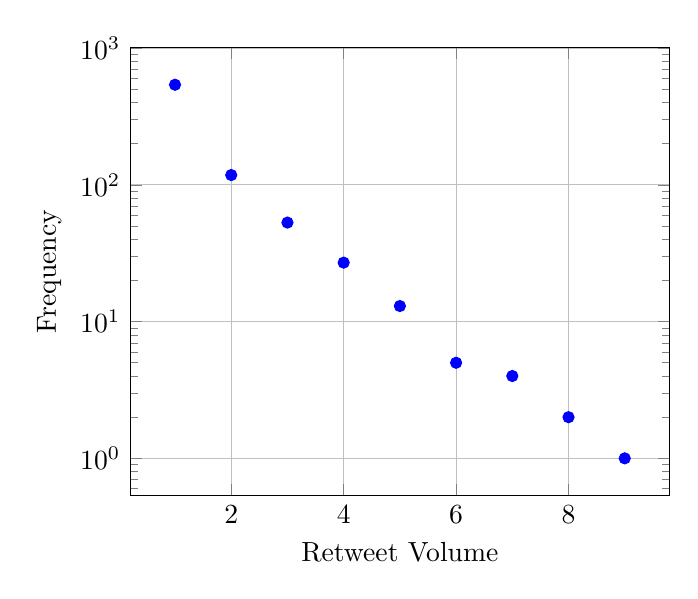
\begin{tikzpicture}
 \begin{semilogyaxis}[
        xlabel=Retweet Volume,
        ylabel=Frequency,
        grid = major]
    \addplot[only marks,mark=*,blue] plot coordinates {
        (1,540)  (2,118)  (3,53) (4,27) (5,13) (6,5) (7,4) (8,2) (9,1) (10,0)
    };
\end{semilogyaxis}
\end{tikzpicture}
\caption{Retweet volume frequency distribution from path network simulation}
\label{fig:linear}
}
\end{figure}
Figure \ref{fig:linear} shows the frequency distribution for a path network when simulated with the logistic regression over a series of tweets. The graph shows a very large proportion of single retweets, which reduces logarithmically with larger volumes.
\\
The likelihood of a user getting the chance to retweet, and also deciding to retweet, becomes the product of a probability function the further the tweet travels, where user $ N_i $ requires all users $ N_0 $ to $ N_{i-1} $ to pass on the message before it even gets a chance to make the retweet decision.
\\
As a result, if the retweet decision chance of each user is more or less equal, the chance of user $ N_2  $ retweeting the tweet is of an order of magnitude less than that of user $ N_1 $ deciding to retweet. The graph shows half life-style behaviour; owing to the fact that each retweet is exponentially less likely to occur than the previous retweet. Note that the graph is plotted on a log-linear scale.

\subsection{Random Network}
Random networks are more similar to Twitter's own social structure than path networks, but are a much more basic and uniform version and do not consider more influential users or the development of Twitter communities.
\\
A random network is defined as a network of users, $ N $, of size $ n $ in which a user $ N_x $ has probability $ p $ of following user $ N_y $. Thus; as the probability $ p $ is increased, the likelihood of a user following other users in $ N $ increases, causing the overall network edge density to increase. Generally, the average number of followers and followees of a user is proportional to $ p\times n $. Thus the parameters for constructing such a graph are the network size, $n$, and the attachment probability, $p$. The simulation results for the random network indicates a higher distribution of mid-range retweet volumes.
\begin{figure}[h]
\centering{
\begin{tikzpicture}
 \begin{semilogyaxis}[
        xlabel=Retweet Volume,
        ylabel=Frequency,
        grid = major]
    \addplot[only marks,mark=*,blue]
       file {5.Chapter2/data/random.dat};    
\end{semilogyaxis}
\end{tikzpicture}
\caption{Retweet volume frequency distribution from random network simulation}
\label{fig:random}
}
\end{figure}
\subsection{Scale-Free Network}
Include more mathematical analysis of scale-free networks (in general) - i.e., in what way are they logarithmic?
\\
A scale-free network is a network of users, $ N $, of size $ n $ and is generated in such a way so that the resultant distribution of degree follows a power-law. \emph{In}-degree signifies the number of inward edges to a node (i.e. the number of followers of a user), whereas \emph{out}-degree is the number of outward edges (i.e. the number of users that user follows).
\\
Scale-free networks have been the subject of a fair amount of research, and are explained more thoroughly in \cite{hein06}. In our implementation we use NetworkX\footnote{http://networkx.lanl.gov}, a Python networking package, to generate directed scale-free networks through a preferential-attachment algorithm based on the network size and edge density as parameters.
\\
Figure \ref{fig:real-scalefree} shows the frequency distribution of retweet volumes. Since the data is plotted on logarithmic scales, we see a logarithmic trend very similar to our results in \cite{webberley11}.
%\begin{figure}[h]
%\centering{
%\begin{tikzpicture}
% \begin{loglogaxis}[
%        xlabel=Retweet Volume,
%        ylabel=Frequency,
%        grid = major]
%    \addplot[only marks,mark=*,blue]
%       file {data/scale-free.dat};
%    
%\end{loglogaxis}
%\end{tikzpicture}
%\caption{Retweet volume frequency distribution generated in scale-free networks}
%\label{fig:scale-free}
%}
%\end{figure}
\subsection{Comparison to Real Twitter Data}
In our previous work, \cite{webberley11}, we captured and analysed data which contained results on the distribution of retweet group sizes. In that paper, a retweet group was defined to be a set of tweets containing one tweet and then all the retweets of that tweet. Thus the retweet volume looked at in this section is effectively the cardinality of the retweet group (minus one). Since the results in the above experiments also look at the frequency distribution of retweet volumes, then we should be able to draw some comparisons.
\\
We compared the data produced by the different types of network to this previous data, and found that the scale-free network produced a distribution similar to that from the real Twitter data.
\begin{figure}[h]
\centering{
\begin{tikzpicture}
 \begin{loglogaxis}[
        xlabel=Retweet Volume,
        ylabel=Frequency,
        grid = major,
        legend entries={Real data,Scale-free}]
    \addplot[only marks,mark=*,red]
       file {5.Chapter2/data/comparison-real.dat};
    \addplot[only marks,mark=*,blue]
       file {5.Chapter2/data/comparison-scale-free.dat};
\end{loglogaxis}
\end{tikzpicture}
\caption{Comparing the retweet volumes distribution from scale-free graph simulation to data from Twitter's graph}
\label{fig:real-scalefree}
}
\end{figure}

\subsection{Structure Comparison}
Each network structure has been demonstrated to show different propagation characteristics. This has shown that, in addition to a user's own retweet decision, the actual spread of a tweet depends somewhat on how the author's local network is constructed. With lots of edges in the graph, there are many more paths down which propagation can occur, increasing the number of times a retweet decision is made, and therefore an increase in the overall number of retweets occurring. The retweet decision facilitated by the model, therefore, combined with a user network give an overall \textit{retweetability} of a tweet that will vary depending on the network it's being propagated in, the source user, and the intermediary retweeters.
\\
The path network, as designed to be the extreme case, has shown to allow poor propagation. Importantly, whilst the network parameters and retweet decision had to be globally increased to obtain any sensible data from this simulation, the trend still shows how propagation down a single chain isn't hugely effective.
\\
The random network facilitated many more retweets due to the fact that users had a very similar in- and out-degree in all cases across the network. This means that each user is able to receive a lot of information, and is also able to pass on (whether an author or a retweeter) information to lots of users simultaneously in the graph. 
\\ 
Despite random networks supporting large retweet throughput (i.e. high \emph{recall} of information), the disadvantage is that the interest \emph{precision}  is much lower. This is because this type of network relies on users following a large number of other users, thus meaning that they would receive more `noise' (i.e. uninteresting tweets) than if they were more limited and selective. Although tweets that are retweeted are usually of a higher \emph{quality}, not all retweeted tweets will be interesting to all users.
\\
Finally, the scale-free network, whilst not having the highest throughput of information, does have trends most similar to the data on retweet distributions collected from Twitter's social graph. This is due to its ability to emulate more influential users and areas of dense communities (as discussed in \cite{java07}). These networks have the potential to allow for large numbers of retweets, especially if they are sourced from one of these more dense areas, but typically die off more quickly as the tweets are retweeted through less influential users.

\section{Interesting Additional Findings}

\subsection{Graph Density}
Define edge density (with equation

\subsection{Results}
Show links between follower audience -> local network -> density.

\subsection{Uses}
From this data, it is demonstrable that various parameters can be generally successfully inferred from very basic user information.

\section{Predictions From the User Graph}
The final part of this paper focuses on the ongoing development of a method to predict the interestingness of a tweet based on the work in the previous sections. The prediction method, at a high level, compares the predicted retweet outcome of a given tweet to the number of times that tweet has actually been retweeted. If, for example, a tweet is simulated with the help of the model and produces a prediction of two retweets, but the tweet has actually been etweeted four times, then we can infer that this tweet is more interesting (at least, to a subset of users). 
\\
The tweet and user features we looked at earlier in this paper are very static, binary features, which do not take into account the actual content of the text of the tweet. Therefore, if a tweet is retweeted more than was predicted, then there is something in the tweet, such as a link to a particularly interesting article or a breaking news story, that makes it more interesting than the average tweet, with the same binary features, that was used to train the model.
\\
In order to improve the fairness of the experiment, we wanted to ensure that the environment of the tweets (i.e. the user network they are propagated through) is the same as its real-life Twitter counterpart. We could then choose a user, which would become the source user, $U_s$, in the set $U$, and simulate that user's own tweets within their particular local network as described by the model above. This would then produce a retweet volume for this user's tweets, to which we could compare the number of times that tweet has \emph{really} been retweeted.


\subsection{Data Collection}
Due to the exponential scaling properties of Twitter's social graph, it was infeasible to collect any more than two hops away from each user as a representation of that user's local network under the rate limitations of Twitter's REST API. 
\\
In particular, a single Twitter account running an instance of an application was allowed, at the time of these experiments, a maximum of 350 REST API calls per hour. One call would be required, for example, to obtain up to 5000 of the followers of a particular user (i.e. one follower hop from the user). An additional call would then be required to collect each of that user's follower's followers (in order to obtain the \emph{second} hop from the source user). \\
Thus, a user who has 700 followers would require 700 API calls to collect that follower network, in addition to the one required to collect that source user in the first place, and would therefore take over two hours of collection. To collect the \emph{third} hop from the source user would drastically multiply the number of required requests (even if there is significant overlap between the followers) and the time needed. 
\\
If each of the 700 followers of the source user had, on average, 200 followers, then this would require the gathering of $ 700 $ x $200 = 140,000 $ users, equating to more than 402 hours of data collection. Bearing in mind that this would only collect the network features for \emph{one} user, it is clear to see how this is an impractical approach.
\\ \\
Luckily, in \cite{webberley11}, we found that the vast majority of retweets occur \textit{within} two hops of the source user (i.e. a path length of less than three), so we considered that the distance from the source user in each case would be sufficient.
\\
In June 2012, the Twitter REST API was used to conduct a random walk through the social graph. For each user, we collected the most recent 300 tweets (including each tweet's metadata - particularly their retweet count) and their local follower network within two hops. We didn't collect the friend network, as we were only interested in tweets propagating outwards from the source user.
\\
After processing that user, the walker chose a user at random from the present user's set of followers and made this the new current user from which to collect data for. If the present user, at any stage, does not have any followers, a list of previously accepted users is maintained and a follower is chosen from one of those instead.
\\
The walker continued until the rate limit was met, at which time the current state was written to disk, and the walker waited until the rate limit was reset before continuing.
\\
Generally, this resulted in, for each user, a set of up to 300 tweets (totalling to around 10,000 tweets in total) and the network in which these tweets were propagated within. There was no need to collect any further data to train the regression, since we were able to re-use the trained model we used earlier.



\subsection{Validating Results}
Needed to validate results using human input. Machines themselves are generally unable to express human interests, so results need to be properly evaluated.

\subsubsection{Crowdsourcing}
Discuss crowdsourcing, its uses, how it is useful in this area. Talk about its history (with any references), and then about mechanical turk.
\\
Mention mechanics of mechanical turk, how it is US only (but we used crowdflower - which autmatically handles submission to MT and several other crowd-sourcing services.

\subsubsection{What We Wanted to Assess}
Used MK, etc.

\subsubsection{Constructing the Questions}
Set up questions (i.e. 5 tweets - choose most interesting and least interesting), give example of this.


In order to validate our prediction results, we ran a pilot user study in order to obtain some human input on the interestingness of each tweet. We compiled the tweet data into a set of questions which were submitted to Amazon's Mechanical Turk. Each question consisted of five tweets from our dataset and each Mechanical Turk Worker (MTW) undertook five questions. Each question asked the MTWs to select which tweet was the most interesting of the five, and which was the least interesting.
\\
For consistency we ensured that at least three MTWs had answered each question. When selecting tweets to include in the Mechanical Turk questions, we excluded those which are `@-replies' - i.e. tweets which begin with another user's screen-name and typically form part of a conversation between two or more users. This meant that there were around 4,500 tweets in total in the questions.

Through using the model and simulating each user's tweets through their individual local networks we achieved around 86\% accuracy in correctly predicting the number of times each tweet was retweeted. 
\\
The precision in predicting the \textit{interestingness} of each tweet was around 30\%. While this value is low, it does mean that in 30\% of cases, a tweet that we predicted to be interesting was verified to be interesting by at least three MTWs all selecting one tweet from a set of five. In addition, when simulating the questions by randomly choosing the most `interesting' tweet of the five in each case, the performance was unable to near our precision even after several thousand iterations.

\subsection{Improving This}
Need offline methodology.
\\
One route for this would be to try and infer a user's local network from a set of their immediate parameters, drawing on our earlier work suggesting that the Twitter network has the properties of a scale-free small-world graph. Through studying graph patterns, it is possible to make sensible inferences on the edges and nodes of a user's local network based on their follower count. From this, a graph edge density can be calculated, $ d = \frac{|E|}{|N|(|N|-1)} $, for use in generating a scale-free network.
\\
Since, for these preliminary experiments, we were only able to collect data from users with a more modest local network, the real and predicted retweet values were both relatively low, allowing more room for error. When simulating much larger local networks involving many more real retweets for each tweet, predicting interestingness, with some threshold value, may become more accurate and thus help improve the precision. The reason for this is that the retweet count of tweets that naturally get retweeted many tens, hundreds, or more times is likely to vary more with interestingness than those that are naturally only retweeted very few times.

\section{Future Work}
There is much further research that could be carried out based on the results in this chapter. Now that the foundation has been laid for simple retweet prediction based on network analysis, research could begin to look at ways in which, as mentioned, networks could be generated based on a few environmental features surrounding users.
\\
This would allow for quick generation of user networks (bypassing the need for data collection) and would also support the same calculations for more highly influential users (users with more followers and more retweets per Tweet).
\\ \\
For this research, the notion of the network will continue and form the basis of the environmental features in the next chapter. Since we now know that the network plays an important role in dictating the way in which information can propagate

\section{Summary}
In this chapter we aimed to carry out a study on the behaviour of propagation through different types of social graph structures and to introduce our ongoing work into predicting the interestingness of tweets from their retweet patterns.
\\
Using a set of tweet and user features, we trained a regression model which we used to simulate a number of tweets through different network types. We produced a distribution of retweet volumes for each network type and confirmed that, with the same tweet features, different network configurations do indeed facilitate different retweet behaviours in terms of propagation spread. We were also able to compare our results to data from Twitter to verify that Twitter's own social graph most closely resembles a scale-free small world graph.
\\
We then finished by discussing how we used the trained model to simulate real networks from Twitter, along with the tweets that were passed through these networks, in order to try to predict how interesting a tweet is based on its retweet patterns. While we were able to often correctly predict the retweet outcome of a tweet, we found that more work would be required to improve the performance of predicting whether or not these tweets are truly interesting to users.